% !TeX program = xelatex
% Journal-style author manuscript, not an official publisher class.
% Compile main.tex from this directory with XeLaTeX (twice) or Tectonic.
\documentclass[UTF8,a4paper,twocolumn,fontset=none,zihao=5]{ctexart}
\usepackage[top=20mm,bottom=20mm,left=18mm,right=18mm,columnsep=7mm]{geometry}
\usepackage{amsmath,amssymb,booktabs,graphicx,tabularx,array,longtable}
\usepackage{caption,enumitem,needspace,balance}
\usepackage{cite}
\newcommand{\upcite}[1]{\textsuperscript{\cite{#1}}}
\usepackage{xurl}
\usepackage[hidelinks,bookmarksnumbered]{hyperref}
\IfFontExistsTF{SimSun}{\setCJKmainfont{SimSun}[AutoFakeBold=2]}{\setCJKmainfont{FandolSong-Regular}[BoldFont=FandolSong-Bold]}
\IfFontExistsTF{SimHei}{\setCJKsansfont{SimHei}[AutoFakeBold=2]}{\setCJKsansfont{FandolHei-Regular}[BoldFont=FandolHei-Bold]}
\IfFontExistsTF{SimSun}{\setCJKmonofont{SimSun}}{\setCJKmonofont{FandolSong-Regular}}
\setmainfont{texgyretermes-regular.otf}[BoldFont=texgyretermes-bold.otf,ItalicFont=texgyretermes-italic.otf,BoldItalicFont=texgyretermes-bolditalic.otf]
\setsansfont{texgyreheros-regular.otf}[BoldFont=texgyreheros-bold.otf]
\ctexset{section={format=\large\sffamily\bfseries,beforeskip=9pt,afterskip=5pt},
 subsection={format=\normalsize\sffamily\bfseries,beforeskip=7pt,afterskip=3pt}}
\setlength{\parindent}{2em}
\setlength{\parskip}{0pt}
\linespread{1.04}
\setlength{\abovedisplayskip}{5pt plus 1pt minus 1pt}
\setlength{\belowdisplayskip}{5pt plus 1pt minus 1pt}
\setlength{\textfloatsep}{10pt plus 2pt minus 2pt}
\setlength{\dbltextfloatsep}{10pt plus 2pt minus 2pt}
\setlength{\floatsep}{8pt plus 2pt minus 2pt}
\renewcommand{\topfraction}{0.93}
\renewcommand{\dbltopfraction}{0.93}
\renewcommand{\textfraction}{0.06}
\renewcommand{\floatpagefraction}{0.80}
\renewcommand{\dblfloatpagefraction}{0.80}
\setcounter{topnumber}{3}
\setcounter{dbltopnumber}{3}
\makeatletter
\setlength{\@fptop}{0pt}
\setlength{\@fpsep}{10pt}
\setlength{\@fpbot}{0pt plus 1fil}
\makeatother
\captionsetup{font=small,labelsep=quad,skip=4pt}
\setlist[enumerate]{leftmargin=1.8em,nosep,label=\arabic*.}
\newcolumntype{Y}{>{\centering\arraybackslash}X}
\newcommand{\algtitle}[1]{\par\Needspace{6\baselineskip}\smallskip\noindent\textbf{#1}\par\smallskip}
\emergencystretch=1em
\raggedbottom
\pagestyle{plain}
\setcounter{section}{-1}
\hypersetup{pdftitle={资源匹配下超图支付网络的服务可靠性},pdfauthor={作者待填}}


\begin{document}\onecolumn\renewcommand{\thefigure}{S\arabic{figure}}\renewcommand{\thetable}{S\arabic{table}}

\section*{补充分析：直接增量、服务成本、窗口与初态}

本材料整合S1–S5已完成的补充分析。正式、确认标签只指数据来源；这些事后分析不属于原40项预定确认比较，不是新的盲确认。每相位、每规模独立n=60父图，3模型各20；7条轨迹在父图内汇总，同分布4条、偏移3条。模型等权、父图分层整图配对重抽样均为20\,000次；两相位不合并。重抽样副本和请求数不是独立样本数。

S1在两相位16项比较上作Bonferroni名义家族95\%分配，单个区间为99.6875\%；S2无新区间，S3–S5为未校正点态95\% percentile区间，无p值。区间为经验近似，不保证有限样本精确覆盖。所有数据已作单独算术实现核验，该核验不是独立盲科学审查。

\section*{S1：原优化初态的DA减FHS5}

\begin{table}[ht]\centering\caption{全部16项直接比较。Y差为无量纲，F差为百分点；Y正、F负对DA有利。区间均含或触0，退化区间不证明总体等效。}\small\begin{tabular}{llrrrr}\toprule 相位 & n & $\Delta Y$ & 校正区间 & $\Delta F$/pp & 校正区间/pp\\\midrule

正式 & 30 & 0.001858 & [0.000000, 0.004802] & 0.000000 & [0.000000, 0.000000] \\

正式 & 60 & 0.000086 & [0.000000, 0.000417] & -0.238095 & [-1.190476, 0.000000] \\

正式 & 120 & -0.000084 & [-0.000422, 0.000000] & 0.000000 & [0.000000, 0.000000] \\

正式 & 240 & 0.000000 & [0.000000, 0.000000] & 0.000000 & [0.000000, 0.000000] \\

确认 & 30 & 0.000906 & [0.000000, 0.002851] & -1.190476 & [-3.571429, 0.000000] \\

确认 & 60 & -0.000152 & [-0.000694, 0.000000] & 0.000000 & [0.000000, 0.000000] \\

确认 & 120 & 0.000043 & [0.000000, 0.000215] & 0.000000 & [0.000000, 0.000000] \\

确认 & 240 & 0.000000 & [0.000000, 0.000000] & 0.000000 & [0.000000, 0.000000] \\

\bottomrule\end{tabular}\end{table}

未校正与校正区间均保存在完整源数据中；只报告有利点估计会夸大证据。S5中的原优化拓扑差点估计与此一致，但S5只用点态95\%区间，不能交换显著性口径。

\clearpage

\section*{S1读图：增量与校正家族}

\begin{center}

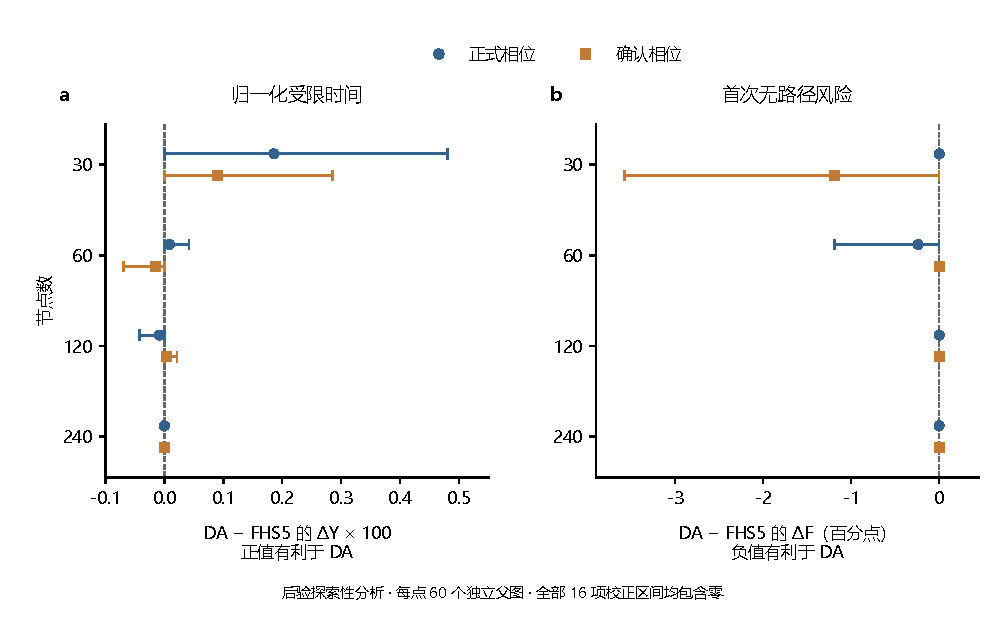
\includegraphics[width=170mm,height=195mm,keepaspectratio]{figures/s1-direct.pdf}

\captionof{figure}{DA减FHS5的直接增量。两面板为Y差乘100（窗口百分数）与F差（百分点）；相位按图内颜色和标记编码。中心为60父图的等模型均值差，线段为16项Bonferroni分配的99.6875\%区间；虚线为0。全部16项保留。图用于判断搜索增量，而非超图与二元参照的主效果。}

\end{center}

\clearpage

\section*{S2：负载范围的描述分解}

每个终点的合并差等于$(4D_{\rm same}+3D_{\rm shift})/7$。下表保留16个相位、规模及终点条件的范围均值，完整112个机制均值在源JSON。没有新增范围区间或交互检验。

\begin{table}[ht]\centering\caption{DA减FHS5的全部范围分解；F差为百分点，Y无量纲。}\small\begin{tabular}{llrrrr}\toprule 相位 & n & 终点 & 同分布 & 偏移 & 合并\\\midrule

正式 & 30 & Y & 0.003252 & 0.000000 & 0.001858 \\

正式 & 30 & F/pp & 0.000000 & 0.000000 & 0.000000 \\

正式 & 60 & Y & 0.000006 & 0.000193 & 0.000086 \\

正式 & 60 & F/pp & 0.000000 & -0.555556 & -0.238095 \\

正式 & 120 & Y & -0.000214 & 0.000089 & -0.000084 \\

正式 & 120 & F/pp & 0.416667 & -0.555556 & 0.000000 \\

正式 & 240 & Y & 0.000000 & 0.000000 & 0.000000 \\

正式 & 240 & F/pp & 0.000000 & 0.000000 & 0.000000 \\

确认 & 30 & Y & 0.001134 & 0.000602 & 0.000906 \\

确认 & 30 & F/pp & -1.250000 & -1.111111 & -1.190476 \\

确认 & 60 & Y & -0.000266 & 0.000000 & -0.000152 \\

确认 & 60 & F/pp & 0.000000 & 0.000000 & 0.000000 \\

确认 & 120 & Y & 0.000075 & 0.000000 & 0.000043 \\

确认 & 120 & F/pp & 0.000000 & 0.000000 & 0.000000 \\

确认 & 240 & Y & 0.000000 & 0.000000 & 0.000000 \\

确认 & 240 & F/pp & 0.000000 & 0.000000 & 0.000000 \\

\bottomrule\end{tabular}\end{table}

相同父图与不同机制之间存在依赖，符号差异不是范围交互证据。原S1和S3历史交付记录中“尚未运行后续”的文字仅表示其封存时点；本版依据后续各自通过核验的归档整合，不回写旧清单。

\clearpage

\section*{S3：累计服务及每成功请求成本}

完整窗口内失败后仍继续支付；S为成功请求数，V为成功金额，C为接受路径的累计暴露。成功比例S/H、金额V/H与首次事件终点不同。成本为$R_C=\mathbb E[C]/\mathbb E[S]$，不是$\mathbb E[C/S]$。每条轨迹内先平均二元参照，再父图内汇总、模型等权；bootstrap内重算各臂比值后相减。64臂单元没有零服务父图/轨迹，320个比值没有未定义重抽样；这些计数完整保留。五成本为经过超边数、信令槽位、独立参与人数、二次暴露及$|e|\log_2|e|$敏感性暴露，均非实测字节、时延、签名或费用。

\begin{center}

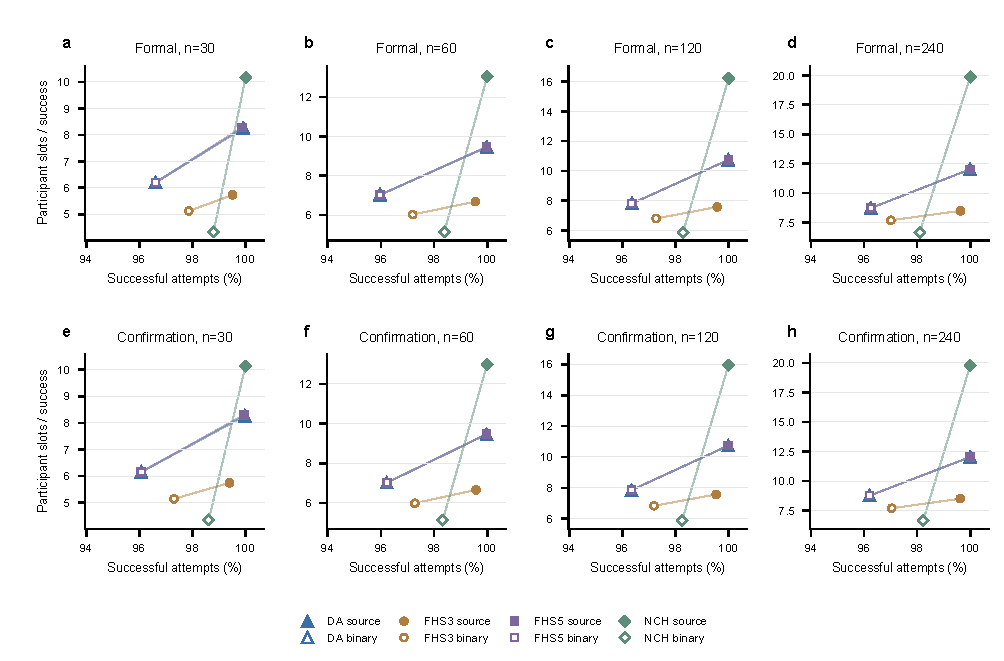
\includegraphics[width=170mm,height=195mm,keepaspectratio]{figures/s3-service-cost.pdf}

\captionof{figure}{服务与信令成本联合描述。8个面板按相位与规模分组，颜色和形状对应4构造，实心/空心区分源超图和自身二元参照，共64个臂单元。线连接同族源与参照，仅表示配对，不是时间轨迹或拟合。横轴为成功请求比例，纵轴为每成功请求信令槽位；竖线为未校正点态95\%区间，横轴未画区间，不是联合95\%区域。各点来自60父图、3模型等权。}

\end{center}

\clearpage

\begin{center}

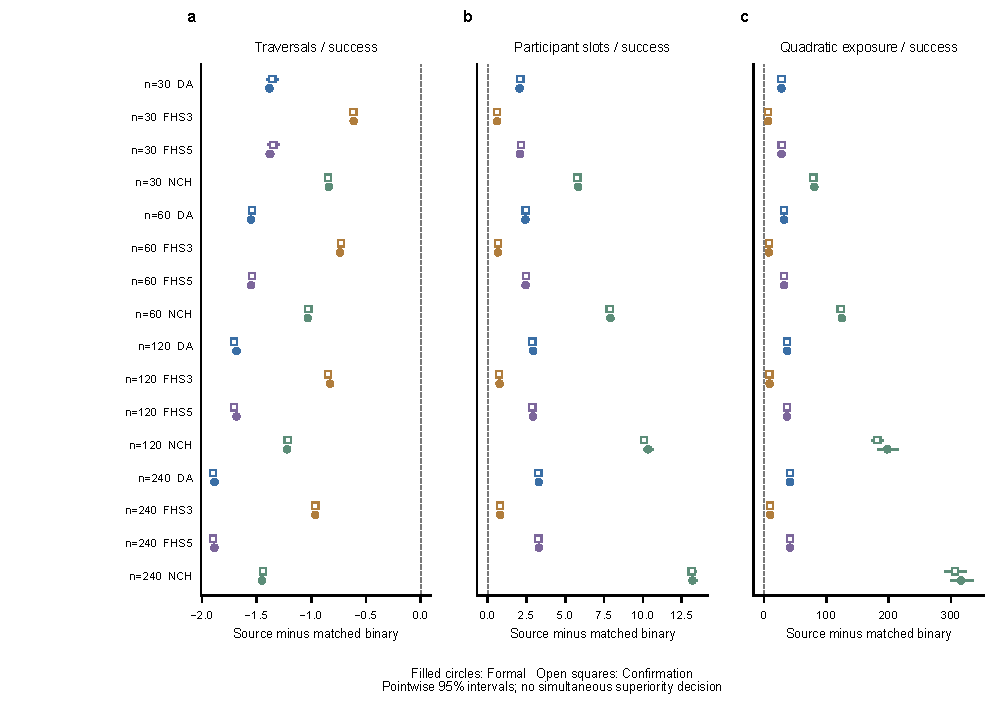
\includegraphics[width=170mm,height=195mm,keepaspectratio]{figures/s3-paired-cost.pdf}

\captionof{figure}{每成功请求成本的配对差。三个面板分别为经过超边数、信令槽位、二次协调暴露量；形状/填充区分相位。全部4构造、4规模、2相位的96项所示成本差保留；完整5成本共200项保存在源JSON。线段为父图分层配对、重新计算均值之比的未校正点态95\%区间，不是比值的均值或差值之比。}

\end{center}

\clearpage

\section*{S4：嵌套窗口敏感性}

从原记录$T=\min(\tau,H)$、$\delta=\mathbf1\{\tau\le H\}$得到$T_h=\min(T,h)$、$\delta_h=\delta\mathbf1\{T\le h\}$、$Y_h=T_h/h$；先逐臂截断再形成参照均值与配对差。整数离散时间满足$\mathbb E[\min(\tau,h)]=\sum_{j=0}^{h-1}\Pr(\tau>j)$。末次事件与无事件可能同为$Y_h=1$，但风险不同。160窗口效应和80直接窗口变化区间均为点态、未校正95\%；320子范围效应和160子范围变化只有描述值。本分析不产生前缀成本、未删失寿命或规模与时域的因果分解。

\begin{center}

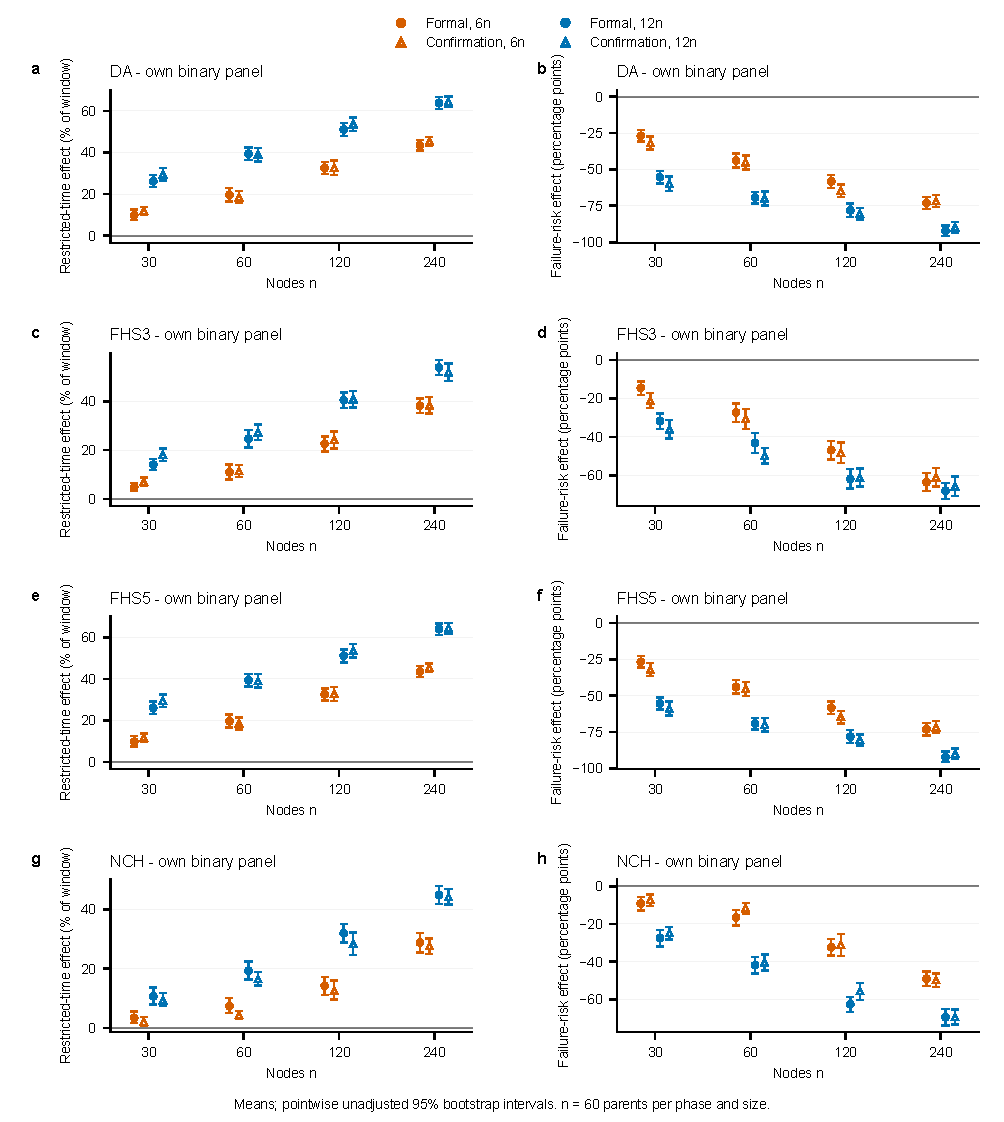
\includegraphics[width=170mm,height=195mm,keepaspectratio]{figures/s4-binary-window.pdf}

\captionof{figure}{窗口敏感性的超图减自身二元参照比较。4行构造、2列终点；颜色表示6n/12n窗口，形状表示相位。左列Y差乘100（窗口百分数），右列F差为百分点，不能互换单位。全部两窗口、两相位、4规模、4构造均保留。每条件60父图，区间为未校正点态95\%；不是同时置信保证。}

\end{center}

\clearpage

\begin{center}

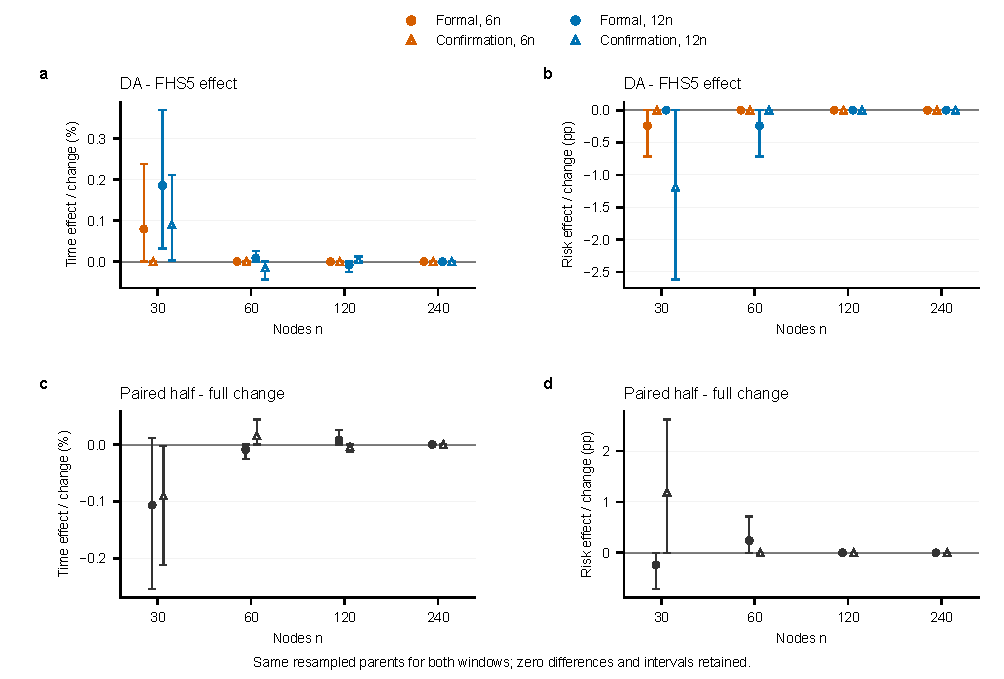
\includegraphics[width=170mm,height=195mm,keepaspectratio]{figures/s4-direct-window.pdf}

\captionof{figure}{DA减FHS5的窗口效应和直接变化。上排为两个窗口的终点差，下排为6n减12n配对变化；左列Y差乘100，右列F差为百分点，按图内颜色、形状区分窗口和相位。变化区间用共享父图重抽样直接计算，不能由两个区间端点相减。每条件60父图，未校正点态95\%；零宽区间不证明总体等效。}

\end{center}

\clearpage

\section*{S5：四臂资金初态比较}

节点预算120不变，拓扑DA/FHS5固定，U均匀、O原优化，复用相同留出请求和路由票据。每相位每规模20\,000次共享索引重抽样；80合并对比有点态95\%未校正区间，160子范围对比无区间，192绝对均值全部保留。种子2026100705按SHA-256派生，点态区间取第500与第19\,500顺序统计量。资金重新分配可改变每条超边总资金，不是固定超边资金的纯拓扑干预。

\begin{center}

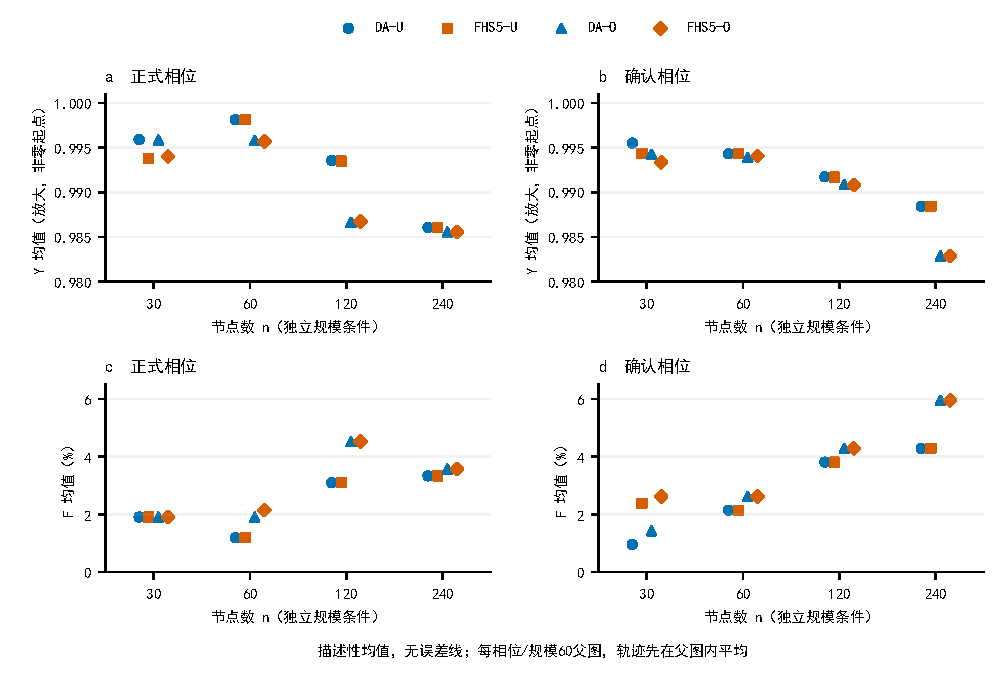
\includegraphics[width=170mm,height=195mm,keepaspectratio]{figures/s5-arm-means.pdf}

\captionof{figure}{四臂绝对均值。a、b为正式与确认相位Y均值，c、d为F均值（百分数）。Y轴非零起点放大，F轴从零开始；不画误差线。每条件60父图，7轨迹父图内汇总、3模型等权。U为节点预算均匀初态、O为原优化初态。标记表示离散规模条件，不是时间轨迹；绝对水平不证明臂间等效。}

\end{center}

\clearpage

\begin{center}

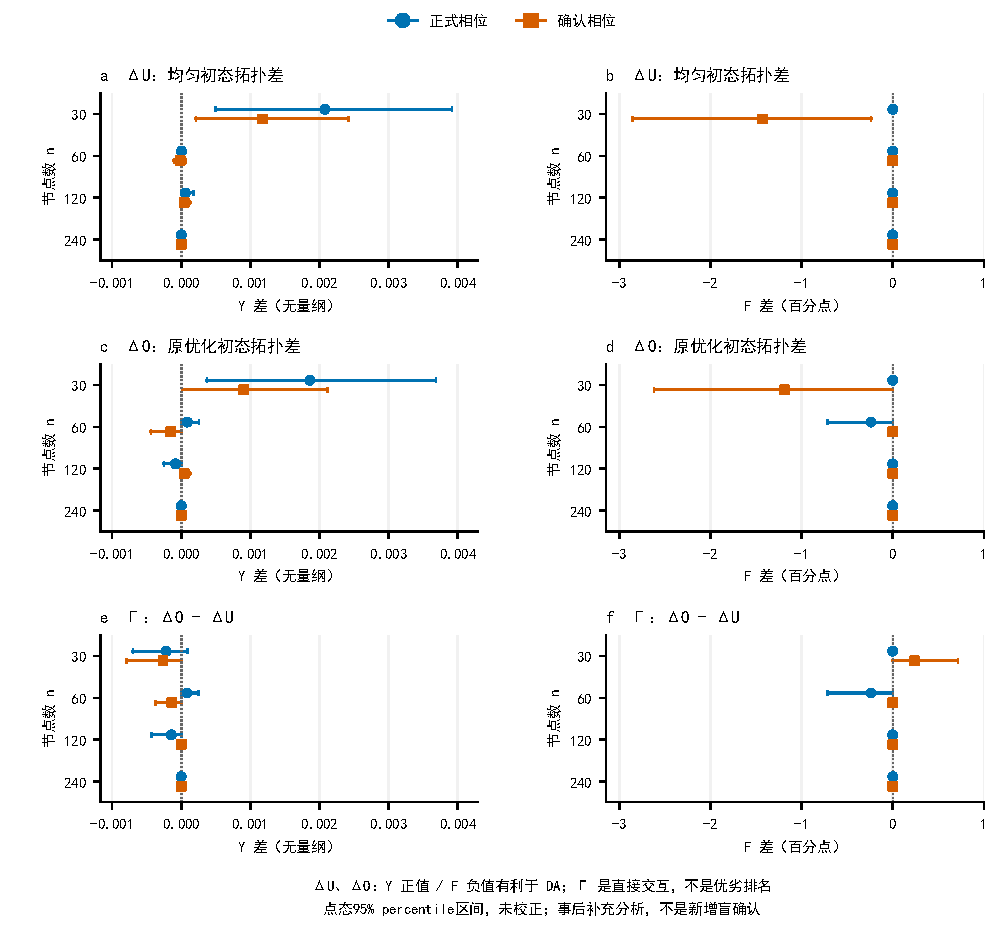
\includegraphics[width=170mm,height=195mm,keepaspectratio]{figures/s5-topology-interaction.pdf}

\captionof{figure}{四臂拓扑差与直接交互。a、b为U初态DA减FHS5，c、d为O初态，e、f为两拓扑差之差；左列Y差，右列F差（百分点）。圆点为正式、方块为确认。共48项合并比较，线段为每条件60父图的共享索引配对未校正点态95\%区间；交互不由一项显著另一项不显著推断。}

\end{center}

\clearpage

\begin{center}

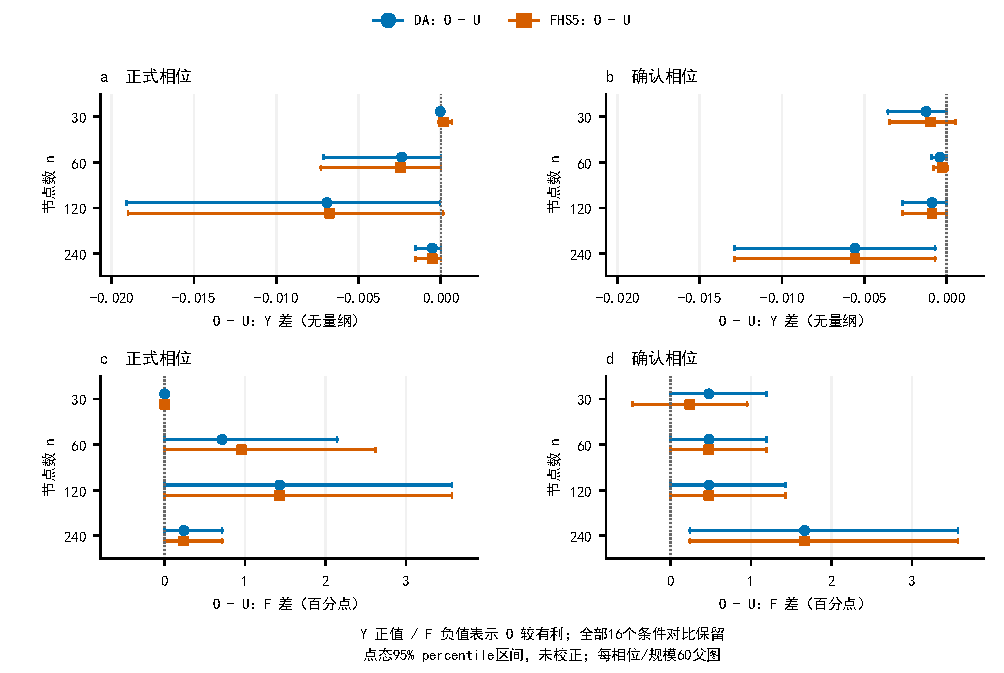
\includegraphics[width=170mm,height=195mm,keepaspectratio]{figures/s5-initialization.pdf}

\captionof{figure}{固定拓扑内O减U。a、b为两相位Y差，c、d为F差（百分点）。圆点为DA、方块为FHS5，共32项合并比较，线段为未校正点态95\%区间。每条件60父图，Y正、F负表示O有利。16个时间条件15负1正仅为方向计数。此图为正文初态对比的完整显示。}

\end{center}

\paragraph{复用与溯源} 图均逐字节沿用已核验PDF，未改变点、区间或坐标。全部源JSON、核验收据、完整图表和计算检查点仍存仓库；附作者包包含完整统计JSON，输入清单及SHA-256另列。原稿中13项描述指标的完整定义仍保留在原随稿补充说明。图S1–S8为本版统一图号，S1–S5为分析标识；二者不同。

\end{document}
